\begin{figure}[htbp]
    \centering

    \begin{subfigure}[b]{0.23\textwidth}
        \centering
        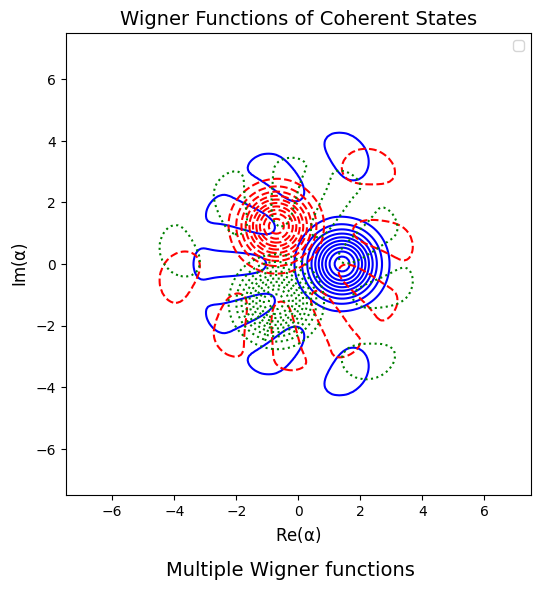
\includegraphics[width=\linewidth]{figures/q3_n3.png}
        \caption{\#qubits = 3}
        \label{fig:coh_q3_n3}
    \end{subfigure}
    \hfill
    \begin{subfigure}[b]{0.23\textwidth}
        \centering
        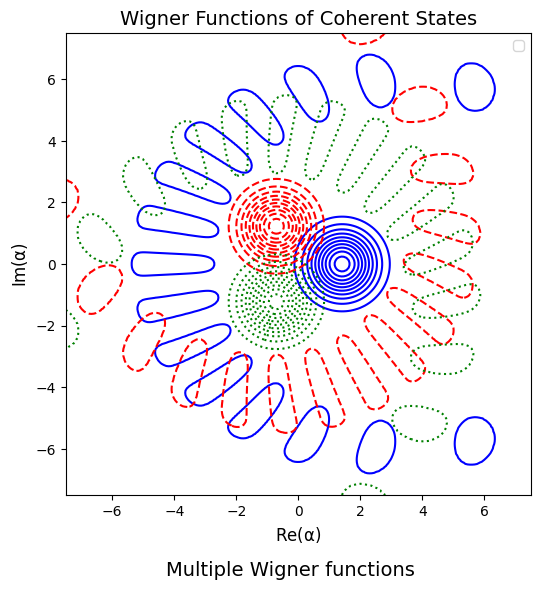
\includegraphics[width=\linewidth]{figures/q4_n3.png}
        \caption{\#qubits = 4}
        \label{fig:coh_q4_n3}
    \end{subfigure}
    \hfill
    \begin{subfigure}[b]{0.23\textwidth}
        \centering
        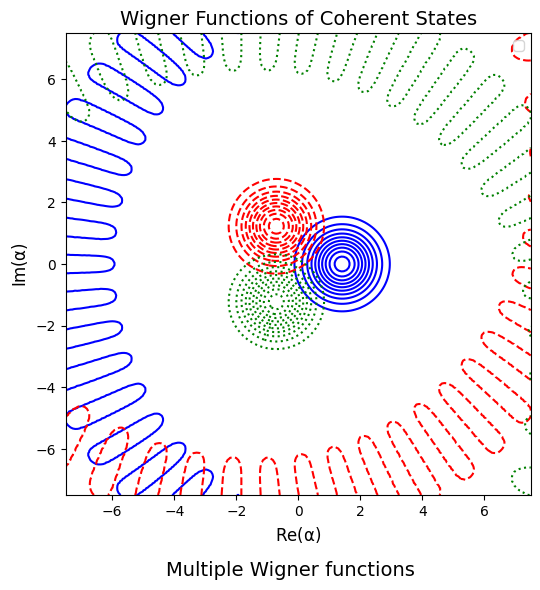
\includegraphics[width=\linewidth]{figures/q5_n3.png}
        \caption{\#qubits = 5}
        \label{fig:coh_q5_n3}
    \end{subfigure}
    \hfill
    \begin{subfigure}[b]{0.23\textwidth}
        \centering
        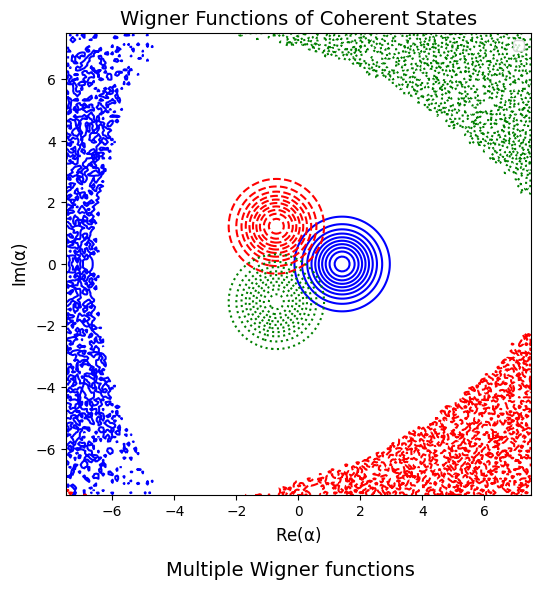
\includegraphics[width=\linewidth]{figures/q6_n3.png}
        \caption{\#qubits = 6}
        \label{fig:coh_q6_n3}
    \end{subfigure}

    \caption{Wigner functions for multiple truncated coherent states with
        different number of qubits. Blue, green, red represent the state
        $\ket{\alpha}$ with
        $\alpha = 0, e^{\frac{2\pi}{3} j}, e^{\frac{4\pi}{3} j}$, respectively.}
    \label{fig:coh_comparison}
\end{figure}